\documentclass{article}



\usepackage[brazil]{babel}

\usepackage[utf8]{inputenc}

\usepackage{amsmath}

\usepackage{amsfonts}



\usepackage[section]{placeins}



\usepackage{graphicx}
\usepackage{booktabs}
\usepackage{multirow}

\usepackage{color} %red, green, blue, yellow, cyan, magenta, black, white

\definecolor{mygreen}{RGB}{28,172,0} % color values Red, Green, Blue

\definecolor{mylilas}{RGB}{170,55,241}



\begin{document}



\begin{flushleft}

\textbf{FUNDAÇÃO GETÚLIO VARGAS} \\



\textbf{Escola de Pós-Graduação em Economia}



\textbf{Teoria Macroeconômica III - Lista 03}



Professor: Ricardo de Oliveira Cavalcanti



Monitora: Kátia Aiko Nishiyama Alves



Alunos: Samuel Barbosa e Gustavo Bulhões

\end{flushleft}



\section*{Exercício 01}

Neste exercício consideramos a economia de trocas estudada por Huggett (1993).



\subsection*{Item (a)}

Utilizando o limite de endividamento $\underline{a} = -2$ e seguindo os demais parâmetros em Hugget (1993), obtemos as seguintes funções valor e política nos estados $e_H$ e $e_L$:



\begin{figure}[!h]

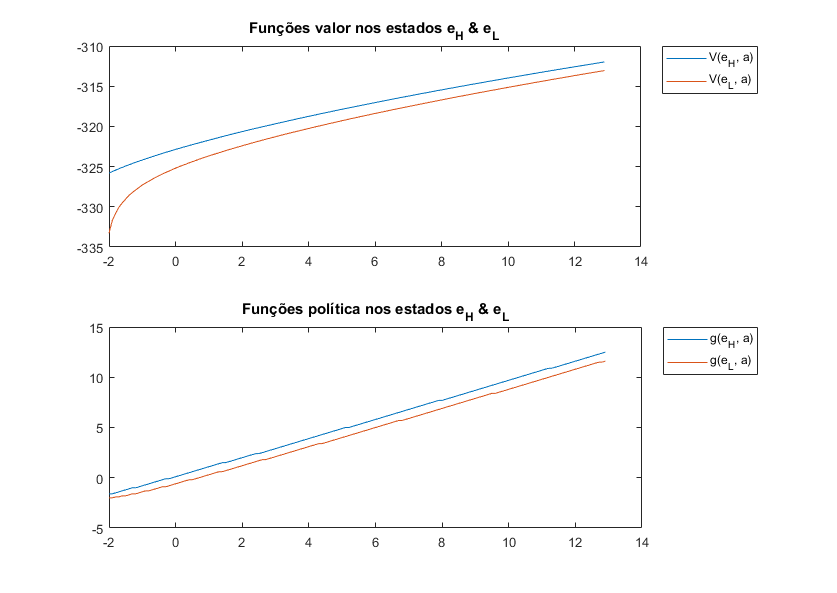
\includegraphics[scale=0.6]{ex1/ex1_1.png}

\end{figure}



\subsection*{Item (b)}



Código anexo.



\subsection*{Item (c)}



Observe que $$(M' - 1I) \lambda = 0 \iff M' \lambda = \lambda,$$ isto é, o autovetor associado ao autovalor unitário de $M'$ é uma distribuição invariante de $M'$. Ao normalizar este autovetor, podemos interpretá-lo, no modelo de Huggett, como a probabilidade (ou proporção) estacionária de indivíduos em cada estado $(a, e)$.



\subsection*{Item (d)}



Podemos calcular a distribução invariante de M iterando $\lambda_{j+1} = \lambda_j M$ até obter $\lambda_{j+1} = \lambda{j}$. Como esperado, a distribuição obtida é idêntica à calculada no item anterior.



\subsection*{Item (e)}



Ainda com $\underline{a} = -2$ e definindo o preço inicial do ativo em $q = 1$, obtemos, inicialmente, excesso de oferta de crédito $z =1.4399$.



\subsection*{Item (f)}



Ajustando iterativamente os preços, obtemos equilíbrio com $q = 1.0129$ quando $\underline{a} = -2$.



\subsection*{Item (g)}



A tabela a seguir apresenta os preços de equilíbrio nos estados $e_H$ e $e_L$, para diferentes valores de $\underline{a}$. \\



\begin{center}

\begin{tabular}{cc}

	\hline $\underline{a}$ & $q$ \\ \hline

	-2  &  1.0129 \\

	-4  &  0.9981 \\

	-6  &  0.9951 \\

	-8  &  0.9942 \\

         -10  & 0.9939 \\

         -12  &  0.9937 \\ \hline

\end{tabular}

\end{center}

\newpage
\section*{Exercício 02}

Neste exercício consideramos a economia descrita em Imrohoroglu (1992). Seguindo os passos descritos na seção 3 do artigo, conforme código anexo, reproduzimos os resultados da Tabela 1. $\Pi$ representa as diferentes taxas de inflação, e entre parênteses reportamos os desvios-padrão obtidos. 

\begin{center}

{ % begin box to localize effect of arraystretch change
\renewcommand{\arraystretch}{1.25}
\begin{table}[htbp]
  \centering
    \begin{tabular}{rccc}
    \toprule
          & $\Pi = 0.0125$  & $\Pi = 0.0062$  & $\Pi = 0.0000$ \\
    \midrule
    \multirow{2}[1]{*}{Average real cash balances } & 11.014 & 14.852 & 22.844 \\
          & (0.3444) & (0.4649) & (0.7232) \\ \\
    \multirow{2}[0]{*}{Average consumption } & 0.9403 & 0.9401 & 0.9400 \\
          & (0.1107) & (0.0959) & (0.0750) \\ \\
    \multirow{2}[0]{*}{Average income } & 0.9400 & 0.9400 & 0.9400 \\
          & (0.2035) & (0.2035) & (0.2035) \\ \\
    Average utility  & -0.0817 & -0.0765 & -0.0707 \\
    \bottomrule
    \end{tabular}%
  \label{tab:addlabel}%
\end{table}%
} % end box

\end{center}



\section*{Exercício 03}

Neste exercício consideramos a economia descrita em Aiyagari (1994).

\subsection*{Item (a)}

Neste cenário, encontramos a taxa de juros de equilíbrio $r=0.0813$.

\subsection*{Item (b)}

No equilíbrio anterior tínhamos $r=0.0813$, $K=7.1567$ e $w=1.4779$. Com a mudança, encontramos $r=0.0802$, $K=5.3166$ e $w=1.4892$. A nova matriz de transição da produtividade da economia possui uma distribuição invariante com maior proporção da força de trabalho de baixa produtividade. Dessa forma, no equilíbrio, os trabalhadores passam a ter renda menor e, assim, acumulam menos capital. Logo, o estoque de capital diminui e, pelas condições de otimalidade do problema da firma, a taxa de juros diminui e o salário aumenta. 

\subsection*{Item (c)}

O novo equilíbrio é $r=0.2396$, $K=1.3225$ e $w=0.8047$. Com uma depreciação maior, o benefício de acumular capital se reduz. Isso faz com que, no equilíbrio, o estoque de capital seja menor. Logo, pelas condições de otimalidade do problema da firma, a taxa de juros aumenta e o salário diminui. 

\end{document}
